\documentclass[11pt,a4paper]{article}
\usepackage{zws_companion_style}
\usepackage{longtable}
\usepackage[section]{placeins}
\hypersetup{pdftitle={Supplementary Information: Zero Without Stasis: Organisational Emergence in an Exactly Reversible Signed-Charge-Conserving Block Cellular Automaton},pdfauthor={Chris Bartlett},pdfsubject={Supplementary information on reversible signed-charge-conserving block dynamics},pdfkeywords={reversible cellular automata, signed charge, finite-time domain formation}}
\graphicspath{{figures/}}
\newcommand{\code}[1]{\texttt{#1}}
\renewcommand{\zwsrunninghead}{Supplementary Information}

\begin{document}
\zwstitleblock{Supplementary Information}{Zero Without Stasis: Organisational Emergence in an Exactly Reversible Signed-Charge-Conserving Block Cellular Automaton}{Chris Bartlett, {\itshape Independent Researcher}. ORCID: \href{https://orcid.org/0009-0001-3323-0131}{0009-0001-3323-0131}\\[1pt]
Supplement to the companion paper, version 1.49, 13 October 2026. DOI: \href{https://doi.org/10.5281/zenodo.22270456}{10.5281/zenodo.22270456}\\[1pt]
Working paper.\\[1pt]
Companion to \emph{Something is happening: Occurrence Theory}, DOI: \href{https://doi.org/10.5281/zenodo.22875288}{10.5281/zenodo.22875288}.}

\tableofcontents

\section{Scope and evidence status}
This Supplement documents the frozen model, the provenance of the selected rule, exact audits, confirmatory measurements, mechanism constraints, and the failure of the later v0.3.2 history-erasure endpoint.

Four evidence classes are kept distinct:
\begin{enumerate}
\item \textbf{Discovery:} a tiny smoke search and its exploratory winner run.
\item \textbf{Confirmation:} frozen-rule repeats and the large exact reversal.
\item \textbf{Mechanism constraints:} density, finite-size, geometry, arrangement, matched-sibling, and ablation comparisons.
\item \textbf{Classifier diagnostics:} v0.3.2 results that diagnose a failed endpoint rather than answer the intended causal question.
\end{enumerate}

\section{Automaton definition}
\subsection{Alphabet and observables}
The four cell states are empty ($0$), positive excitation ($+$), negative excitation ($-$), and bound-neutral excitation ($\mathrm b$). For a lattice state $x$,
\begin{align}
Q(x)&=N_{+}(x)-N_{-}(x),\\
M(x)&=N_{+}(x)+N_{-}(x)+N_{\mathrm b}(x).
\end{align}
$Q$ is a signed additive charge. $M$ counts non-empty cells and is called occupancy or material in the software. The selected rule conserves $Q$ in every local block update but not $M$. All principal worlds were initialised in the global $Q=0$ sector. The phrase ``$Q=0$ sector'' must not be read as ``the rule conserves the value zero only'', ``$Q$ and $M$ both vanish'', or ``the world is empty''.

\subsection{Block code and phase schedule}
On a periodic $H\times W$ lattice with even dimensions, alternating $2\times2$ Margolus partitions cover the lattice. Each four-cell block is packed in base four to an integer in $[0,255]$. A permutation $f$ of those 256 codes supplies the forward update; $f^{-1}$ supplies the inverse. The partition phase is part of the dynamical state. Exact reversal applies the inverse table while stepping phases in reverse order.

\begingroup\sloppy The frozen table is stored in \path{extensions/reversible_null_phase/rules/}\allowbreak\mbox{\path{winner_d1fe99.json}}. SHA-256 of the raw 256 unsigned-byte table, not the JSON serialisation, is\par\endgroup
\begin{center}
\code{d1fe99b5735d8e9be032347de2727dc5c52a7848df200ca26f67f28c8c1bc41c}.
\end{center}
The rule is a permutation; all 256 outputs are unique. Exhaustive enumeration verifies $Q(f(b))=Q(b)$ for every block state $b$. The same enumeration finds block states for which $M(f(b))\ne M(b)$.

The block code uses the digits $0$ (empty), $1$ ($+$), $2$ ($-$) and $3$ ($\mathrm b$) in base-four order top-left, top-right, bottom-left, bottom-right,
\begin{equation}
c=s_{\mathrm{TL}}+4s_{\mathrm{TR}}+16s_{\mathrm{BL}}+64s_{\mathrm{BR}}.
\end{equation}
The construction starts from clockwise block rotation and exchanges 12 reversible output pairs; consequently, 24 of 256 inputs differ from the rotation scaffold. Two entries used in the main-text worked diagram are exact table values. Entry $f(1)=4$ maps $(+,0;0,0)$ to $(0,+;0,0)$ and preserves $(Q,M)=(+1,1)$. Entry $f(130)=154$ maps $(-,0;0,-)$ to $(-,-;+,-)$ and changes $(Q,M)$ from $(-2,2)$ to $(-2,4)$: one positive and one negative excitation are added as a balanced pair. The inverse permutation maps code 154 back to code 130. These examples illustrate transport and reaction channels; they are not a claim that either lookup alone is sufficient for the macroscopic behaviour.

\section{Rule discovery and selection accounting}
\subsection{What was searched}
The historical discovery metadata records construction family \code{reactive\_rotation}, elite source \code{g0000\_reactive12}, final rank zero, 12 swaps, 14 unique rules evaluated, and 16 replicate rule evaluations. The search run was a smoke-scale campaign. It was not a representative sample of the enormous permutation space (the metadata records the base-10 logarithm of the rule-space size as approximately 317.961), and the selected rule must be described as search-selected.

\subsection{Declared score}
For each candidate, the software averaged activity, reaction density, state entropy, block entropy, spatial mutual information, temporal mutual information, recurrence, and perturbation distance over sampled phases and measured repeated $4\times4$ patches. A weighted sum rewarded broad intermediate target bands:
\begin{center}
\begin{tabular}{@{}lr@{}}
\toprule
Term & Weight \\
\midrule
Activity & 0.14 \\
Reaction density & 0.11 \\
State entropy & 0.11 \\
Block entropy & 0.11 \\
Spatial mutual information & 0.14 \\
Temporal mutual information & 0.14 \\
Recurrence & 0.10 \\
Perturbation distance & 0.09 \\
Patch repetition & 0.06 \\
\bottomrule
\end{tabular}
\end{center}
A sigmoid gate penalised insufficient activity and reaction, and any failure of charge preservation was given a sentinel score. The exact bands and softness parameters are in \code{src/\allowbreak zws\_nullity\_lab/\allowbreak metrics.py}. The search therefore selected for lively, structured, non-trivial dynamics. It did not select on large-lattice reversal, strong-domain first passage, density dependence, finite-size scaling, event morphology, prepared geometry, double conservation, reaction-pair ablation, prevalence, or history-erasure diagnostics.

\subsection{Evidence matrix}
\begin{longtable}{@{}>{\raggedright\arraybackslash}p{0.19\linewidth}>{\raggedright\arraybackslash}p{0.22\linewidth}>{\raggedright\arraybackslash}p{0.23\linewidth}>{\raggedright\arraybackslash}p{0.24\linewidth}@{}}
\caption{Evidence matrix: the frozen object, principal output and warranted inference of each stage.}\label{tab:evidence-matrix}\\
\toprule
Stage & Frozen object & Principal output & Valid inference \\
\midrule
\endfirsthead
\toprule
Stage & Frozen object & Principal output & Valid inference \\
\midrule
\endhead
Discovery & small reactive-rotation search & selected winner from 14 unique candidates / 16 replicate evaluations & provenance only; selected behaviour \\
Confirmation & winner, large torus, inverse schedule & $4096^2$, 65,536 forward phases, zero mismatches after inversion & exact implementation-level coexistence of reversal and structure \\
Repeat runs & winner, four localised-patch seeds & transient scale peak 72.66--136.11$\times$ & reproducible large finite-time transient \\
Composition & frozen state summaries & occupancy 0.572989; normalised entropy 0.946343 & local state diversity survives macrostructure \\
Density & seven initial occupancies & event fraction and survival shift strongly with density & finite-time density dependence \\
Morphology & event-centred windows & 67 distributed, 24 unresolved, 0 localised & no support for simple localised-front story \\
Prepared geometry & droplet, slab and homogeneous controls & 0/48 vs 19/24 events by 262,144 phases & relative-growth counts only; different initial baselines, while shapes persist \\
Exact-$Q{+}M$ sibling & reactive matched sibling & 0/16 vs winner 10/16 & nearby double-conservation rule does not reproduce regime \\
Ablations & twelve single-pair removals & 0--7/16 versus winner 10/16 & multiple reaction channels contribute \\
Prevalence & 256 generator draws & 19/256, Wilson 95\% 4.8026--11.3001\% & non-unique within sampled generator only \\
History erasure v0.3.2 & shuffled branches + old endpoint & classifier triggered on shuffled noise & endpoint failure; no causal conclusion \\
\bottomrule
\end{longtable}

\section{Exact reversal and composition}
The large audit used a $4096\times4096$ periodic lattice (16,777,216 cells) with a populated central random patch, not a whole-world homogeneous start. The square patch spans 45\% of each dimension; its target internal proportions are 12\% positive, 12\% negative and 8\% bound-neutral, and the exterior is empty. After 65,536 forward block phases, the run reversed the phase schedule and applied the inverse permutation. The final recovered state was identical to the initial state at every cell. Global signed charge remained $Q=0$. Occupancy $M$ changed during the trajectory, as permitted by the rule.

The four $4096\times4096$ localised-patch confirmation runs supplied the reported median dense-interior occupancy 0.572989 (dense interior: cells in the high-local-density band, excluding a margin around the dense/sparse interface, evaluated at each run's final stored snapshot), positive fraction 0.192542, negative fraction 0.192535, and bound-neutral fraction 0.187912. Normalised four-state entropy was 0.946343. The per-run table behind these medians is included in the release as \path{experiments/domain_mechanism_20260825/artifacts/spatial_reduction/ENVIRONMENT_COMPOSITIONS.csv}: the four \code{stage7b} rows with role group \code{final}, environment \code{dense\_interior}, analysis family \code{density\_robustness}, box width 32 and threshold scheme \code{q20\_q80} reproduce the medians exactly. Those four localised-patch confirmatory winner runs reached transient domain-scale maxima of 72.66--136.11 times their initial scale (median 98.4459); the final stored scales were 15.77--16.33 times initial (median 16.1118). This non-monotonicity is why the paper says ``coarsening-like organisation'' rather than monotonic phase ordering.

\section{Endpoint definitions and initial-condition provenance}
\subsection{Distinct initial-condition families}
The large reversal and the four $4096^2$ growth/composition confirmations use the localised-patch family above. Whole-torus homogeneous-random studies are separate: the principal density map and later first-passage study use $1024^2$ lattices, with smaller $512^2$ comparisons and limited $2048^2$ checks in the recorded campaigns. In the homogeneous density family, an exact inventory with occupied proportions $3/8$ positive, $3/8$ negative and $2/8$ bound-neutral is shuffled over the entire torus. For target occupancy $\rho$ and $N$ sites, the documented rounding is $u=\lfloor\rho N/8+1/2\rfloor$, giving counts $(N-8u,3u,3u,2u)$ of empty, positive, negative and bound-neutral cells. These ensemble constructions must not be pooled as the same initial condition.

\subsection{The implemented v0.3/v0.3.1 endpoint}
Let $a_i(t_j)$ be the areas of finite (non-wrapping) empty components returned by the frozen campaign's four-neighbour toroidal connected-component routine. The characteristic scale is the equivalent-circle radius of the area-weighted mean component area,
\begin{equation}
 L_j=\sqrt{\frac{\sum_i a_i(t_j)^2}{\pi\sum_i a_i(t_j)}}.
\end{equation}
When no finite empty component exists, $L_j=0$. ``Finite'' here excludes winding components; it does not mean that other components contain infinitely many sites on the finite torus. This description does not recompute any campaign.

Set $D=\max(L_0,1)$ and $r_j=L_j/D$. For a prefix through sample $k$, choose $j^*=\min\arg\max_{0\leq j\leq k}r_j$ and let $f_j$ be the largest finite empty component's fraction of all sites. The exact implemented predicate is
\begin{equation}
 C_k=\mathbf{1}[r_{j^*}\geq4\ \wedge\ r_k\geq2\ \wedge\ f_{j^*}\geq0.001
 \ \wedge\ (\forall j\leq k: Q_j=Q_0)].
\end{equation}
In words: take the earliest sample at which the scale ratio reaches its running maximum (the $\min\arg\max$); the flag is true when that peak ratio is at least 4, the current ratio is at least 2, the largest finite empty component at the peak sample covers at least 0.1\% of the sites, and $Q$ has never changed. At least two snapshots are required. The largest-component fraction is evaluated at the \emph{first peak-scale sample}, not necessarily at its own separate maximum. No Fourier, long-wave (low-$k$), entropy or mutual-information threshold enters $C_k$. Those diagnostics are recorded independently. The paper therefore does not describe the endpoint as a joint spectral-and-geometrical test.

For v0.3.1, sampled phases are spaced by 2,048. $T_{\rm hit}$ is the earliest sample with $C_k=1$. $T_{\rm persistent}$ is the earliest start of three consecutive true prefix flags, which can follow an earlier isolated hit. No event time is interpolated between observations; an absent event is right-censored at the trajectory's actual follow-up horizon. The implementation sources are \code{metrics.py:StrongDomainCriterion} and \code{nucleation.py:first\_passage\_from\_flags}, in the computational release identified in the provenance note.

\subsection{Earlier frozen endpoints are not identical}
The original 2026-08-25 confirmation required a final coarse-density dispersion of at least 8 (the variance of the occupied fraction across $64\times64$ blocks divided by the variance a random arrangement of the same cells would give), a final empty-domain scale of at least twice its initial value, a positive fitted late-half scale slope, and exact charge preservation. Its strict sustained-coarsening criterion was not met at the larger scale; the reproduced transient morphology was reported separately.

The later v0.1 homogeneous-density map used a peak scale ratio of at least 4 and a final scale ratio of at least 2, together with a peak largest finite-empty area of at least $\max(64,16\max(A_0,1))$, where $A_0$ is the initial largest finite-empty area, with $Q=0$ at every saved phase. Its \emph{separate} long-wave spectral flag required radial shells $k=1,\ldots,4$ to have peak/final mean-power ratios of at least 4/2 and peak spectral-fraction ratio at least 2. The v0.3 family instead uses the 0.001 lattice-fraction condition above, as explicitly stated in the v0.3.1 preregistration. Thus the approximately 27.5\% estimate is an operational result of that earlier campaign, not a directly interchangeable critical-density estimate. Within a single unchanged endpoint, different time horizons can be compared without any such substitution.

\subsection{Different sources for the main image panels}
The main reversal figure uses localised discovery seed 260824 and an organised intermediate panel at phase 20,480. Its recovered panel displays the phase-zero state whose exact recovery was established by the 65,536-phase inverse audit. The main micro/macro figure instead uses untouched homogeneous $1024^2$ source \code{3cde465f2d2883dd5af4}, initial occupancy 0.20, seed 6203 and phase 311,296. Its nested $64^2$ crop has counts $(1359,899,947,891)$ and normalised single-site entropy 0.987741. This source is distinct from the four localised confirmation runs behind the dense-interior statistic 0.946343. The v0.3.2 causal-endpoint failure does not invalidate a direct image of the untouched source.

\section{Density and first passage}
\begin{table}[h]
\centering
\caption{Frozen finite-ensemble first-passage summary.}
\begin{tabular}{@{}rrrr@{}}
\toprule
Initial occupancy & Events / 12 & KM median (phases) & Follow-up horizon (phases) \\
\midrule
0.16 & 0  & not reached & 262,144 \\
0.18 & 8  & 495,616 & 524,288 \\
0.20 & 12 & 321,536 & 262,144 / 524,288$^{a}$ \\
0.22 & 12 & 206,848 & 262,144 \\
0.24 & 12 & 108,544 & 262,144 \\
0.25 & 12 & 83,968  & 262,144 \\
0.26 & 12 & 65,536  & 262,144 \\
\bottomrule
\multicolumn{4}{@{}p{0.94\linewidth}@{}}{\footnotesize Homogeneous $1024^2$ worlds; Kaplan--Meier median is the first sample at which the estimated survival is at most $1/2$, not the median of observed events alone. $^{a}$At occupancy 0.20, two already-transformed runs retained their 262,144-phase record and ten censored trajectories continued to 524,288. Four of the 0.18 trajectories remained right-censored. Recorded horizons, not an imputed common duration, are shown.}
\end{tabular}

\end{table}

At 0.18, the extended follow-up changed the interpretation of the shorter campaign: events continued to appear late, so a short-horizon fixed threshold could not be retained. Survival curves preserve censoring. The paper does not extrapolate an infinite-time event probability or claim a critical density. Finite-size and area-scaling analyses did not support the simple local-Poisson expectation that was tested, but the available sizes do not establish an alternative asymptotic law.

Event-centred morphology labelled 67 events as distributed (archival code B), 24 as unresolved (code E), and none as localised (code A); the preregistered rubric is summarised in the main text, Section~5.3, on distributed events and the prepared-geometry comparison. The 91 labelled events are the 68 first hits of the primary $1024^2$ cohort and the 23 of the $512^2$ area-scaling cohort. The label is a measured classifier under frozen windows, not an ontological statement about every possible initiation process.

\section{Arrangement and prepared-shape controls}
Prepared droplets and slabs retained or enlarged their imposed geometry but produced zero strong-domain endpoint crossings across 48 trials by 262,144 phases. Matched homogeneous starts produced 19 crossings in 24 trials. These are outcomes of a \emph{relative-growth} assay: the denominator is each trajectory's own initial finite-empty-domain scale. A prepared macroscopic shape is not on the same baseline as random soup. Accordingly, 0/48 is not evidence that seeded organisation failed to form or persist, and this contrast alone does not establish a basin barrier, history inhibition or failure of all compact seeds. The direct measurements of retained geometry remain valid, separately from the endpoint counts.

Earlier arrangement comparisons and phase controls are retained in the experiment reports. Their role is to constrain trivial initialisation artefacts, not to establish a thermodynamic ensemble.

\section{Double conservation and reaction-pair ablations}
The exact-$Q{+}M$ sibling is a distinct permutation whose every local block update preserves both signed charge and occupancy. It was chosen as the closest tested reactive sibling rather than as a universal representative of double-conserving automata. The median across runs of the mean reaction density was 0.01160, close to the winner's 0.01234, so its negative endpoint is not explained by a dead rule. In the focused $1024^2$ comparison (8 replicates) the winner produced 8/8 strong-domain outcomes and the sibling 0/8. In the pooled $512^2$ balanced protocol (16 replicates) the winner produced 10/16 end-of-window strong-domain passes, the sibling 0/16, and pure rotation 0/16. Table~\ref{tab:pooled-controls}, the pooled controls and ablations, counts passes at the end of the observation window, not first passages: in each of two ablations, one run crossed the endpoint earlier and had fallen back below the final scale-ratio threshold by the end of the window.

\begin{table}[h]
\centering
\caption{Pooled matched controls and ablations: end-of-window strong-domain passes ($512^2$, 16 replicates each).}\label{tab:pooled-controls}
\resizebox{\linewidth}{!}{\begin{tabular}{@{}lrrl@{}}
\toprule
Condition & Strong-domain passes & Trials & Interpretation at tested protocol \\
\midrule
Frozen winner (exact $Q$) & 10 & 16 & reference \\
Reactive exact-$Q{+}M$ sibling & 0 & 16 & active, no winner regime \\
Pure rotation & 0 & 16 & transport-only negative control \\
Ablations 01, 11 & 7 each & 16 each & partial retention \\
Ablation 05 & 6 & 16 & partial retention \\
Ablations 08, 09 & 3 each & 16 each & strong attenuation \\
Ablation 06 & 2 & 16 & strong attenuation \\
Ablations 00, 02, 03, 04, 07, 10 & 0 each & 16 each & suppression \\
\bottomrule
\end{tabular}
}
\end{table}

The six zero-pass ablations and the graded intermediate responses support a cooperative reaction architecture. They do not identify a unique minimal causal set because only single-pair removals were tested and finite-horizon zeros are not impossibility theorems.

\section{Prevalence screen}
The generator screen counted 19 strong-domain rules among 256 independent charge-preserving candidates, a sample proportion of 0.074219 and Wilson 95\% confidence interval 0.048026--0.113001. This estimate pertains to the specified generator and protocol. It does not measure the fraction of all local permutations, all charge-preserving permutations, or all rule-construction families. The selected winner remains selected evidence.

\section{Classifier validity under the shuffling intervention}
\subsection{Intended intervention}
The v0.3.2 campaign branched deterministic trajectories at frozen source states. Two branch points were preregistered for each of the 16 source trajectories: Branch A, the first sampled phase at which occupancy reached $M/N\geq0.35$ while the source was still below the endpoint, and Branch B, 32,768 phases before the source's own first hit. Every eligible A and B state received one primary global shuffle, 16 of each. Every B state also received a $32\times32$ and a $128\times128$ tile permutation, four B states received a second global shuffle, and four B states received an even-lattice translation, a null intervention that the dynamics cannot distinguish from the source; so there are 20 Branch-B global shuffles in all, 16 of them primary, and 72 altered branches in total (16 Branch-A shuffles, 20 Branch-B shuffles, 32 tile permutations and 4 translation nulls). Global shuffles and tile permutations preserved each single-site state count, and hence $Q$, $M$ and single-site entropy; both retained the partition phase. The intervention removed spatial arrangement while leaving the subsequent rule deterministic. Every one of 72 altered-branch intervention audits passed. The topology-fixed run is the only valid raw basis; the earlier topology-bug run is excluded.

The intended primary contrast was first passage to the existing strong-domain endpoint after shuffling versus an untouched continuation. This would have been informative only if the endpoint discriminated the organised source geometry from the shuffled geometry.

\subsection{Immediate state audit}
It did not. In Branch A primary global shuffles, mean long-wave power fell from 5,544.267654 to 43.719036: 99.211455\% of the source value was removed. Interface density rose from 0.364832 to 0.455946, anisotropy fell from 0.549951 to 0.159870, and nearest-neighbour mutual information fell from 0.0208694 to approximately $4.05\times10^{-6}$. The intervention therefore did erase measured organisation.

In all 20 Branch-B global shuffles, mean long-wave power fell from 7,246.310873 to 45.649658. Yet 9 of the 16 primary Branch-B replicates were assigned a residual first-passage time $R_{\mathrm{hit}}=0$, 14/16 hit by 4,096 phases, 15/16 by 6,144 phases, and the remaining replicate hit at 20,480 phases. A branch is classified with its source's calibration (the initial finite-empty scale) and the source's prefix history carried forward, so the peak condition is already met when the branch begins and the first branch snapshot can satisfy the current-scale condition on its own; that inheritance is what let a freshly shuffled state register as a hit at elapsed zero. The post-shuffle long-wave mean was only 729.492 at 8,192 phases and 1,127.719 at 16,384 phases, still far below the untouched source's mean. The classifier was therefore responding before long-wave structure had recovered.

\begin{table}[h]
\centering
\caption{Compact audit establishing endpoint failure.}
\resizebox{\linewidth}{!}{\begin{tabular}{@{}p{0.29\linewidth}p{0.29\linewidth}p{0.32\linewidth}@{}}
\toprule
Quantity & Natural source states & Globally shuffled branch states \\
\midrule
Long-wave spectral power, Branch A primary & 5,544.27 (mean) & 43.72 immediately after shuffle \\
Long-wave power removed & -- & 99.21\% \\
Nearest-neighbour mutual information & organised source & approximately $4.05\times10^{-6}$ after shuffle \\
Strong-domain hit at elapsed zero & pre-hit source by branch design & 9/16 Branch B primary replicates \\
Strong-domain hit by 4,096 phases & -- & 14/16 Branch B primary replicates \\
Untouched Branch-A residual record & $R_{\mathrm{hit}}=-28,672$, observed=false & $R_{\mathrm{persistent}}=83,968$ \\
\bottomrule
\multicolumn{3}{@{}p{0.94\linewidth}@{}}{\footnotesize The endpoint's connected-empty-cluster terms can be triggered by random high-occupancy geometry even when long-wave organisation has been destroyed. Therefore the v0.3.2 first-passage comparison is not a valid assay of preserved causal spatial memory.}
\end{tabular}
}
\end{table}

One shuffled state at zero elapsed phases had occupancy 0.409520, histogram (619,163; 145,846; 145,846; 137,721), $Q=0$, long-wave fraction 0.000243482, and nearest-neighbour mutual information approximately $5.57\times10^{-6}$, but nevertheless met the strong-domain endpoint. The finite empty-cluster scale was 157.657 and the largest finite empty component occupied 0.191215 of the lattice. Random high-occupancy geometry can thus create large connected empty components without the organised source's long-wave structure.

\begingroup\sloppy The compact residual-time record also contains a secondary caveat: for source \code{49461bd54e39582ab4fb}, density 0.20, seed 6202, the historical residual-time field \code{untouched\_R\_hit} is $-28,672$ (a bookkeeping field, not an event time) while \code{untouched\_hit\_observed} is false; its persistent residual is 83,968. A negative residual cannot be read as a valid positive post-intervention first-hit time. These historical fields are preserved, not repaired into a new event time. All 72 altered branches ran to their scheduled end, completing the post-event capture window (status \code{post\_persistent\_capture\_complete}); maximum elapsed coverage was exactly $R_{\mathrm{persistent}}+16,384$, where $R_{\mathrm{persistent}}$ is the residual time to the persistent endpoint. The campaign ran as designed. What failed was the classifier's validity for this intervention, not the completeness of the execution.\par\endgroup

\subsection{What the shuffling test does and does not show}
Not shown: that the shuffled branches recovered genuine macroscopic organisation immediately; that hidden multiscale precursor memory was necessary; that erasing history inhibited or accelerated the transition; or that the result established a causal spatial-memory mechanism.

\begingroup\sloppy Directly measured: exact intervention preservation audits; direct evidence that shuffling erased long-wave structure, local mutual information, and anisotropy; deterministic post-intervention trajectories; recovery curves as descriptive dynamics; and the methodological lesson that a connected-cluster endpoint must be revalidated under the intervention's null distribution. The connected-empty-cluster explanation is a diagnostic supported by the observed state geometry, not a proof of equilibrium percolation.\par\endgroup

\begin{figure}[p]
\centering
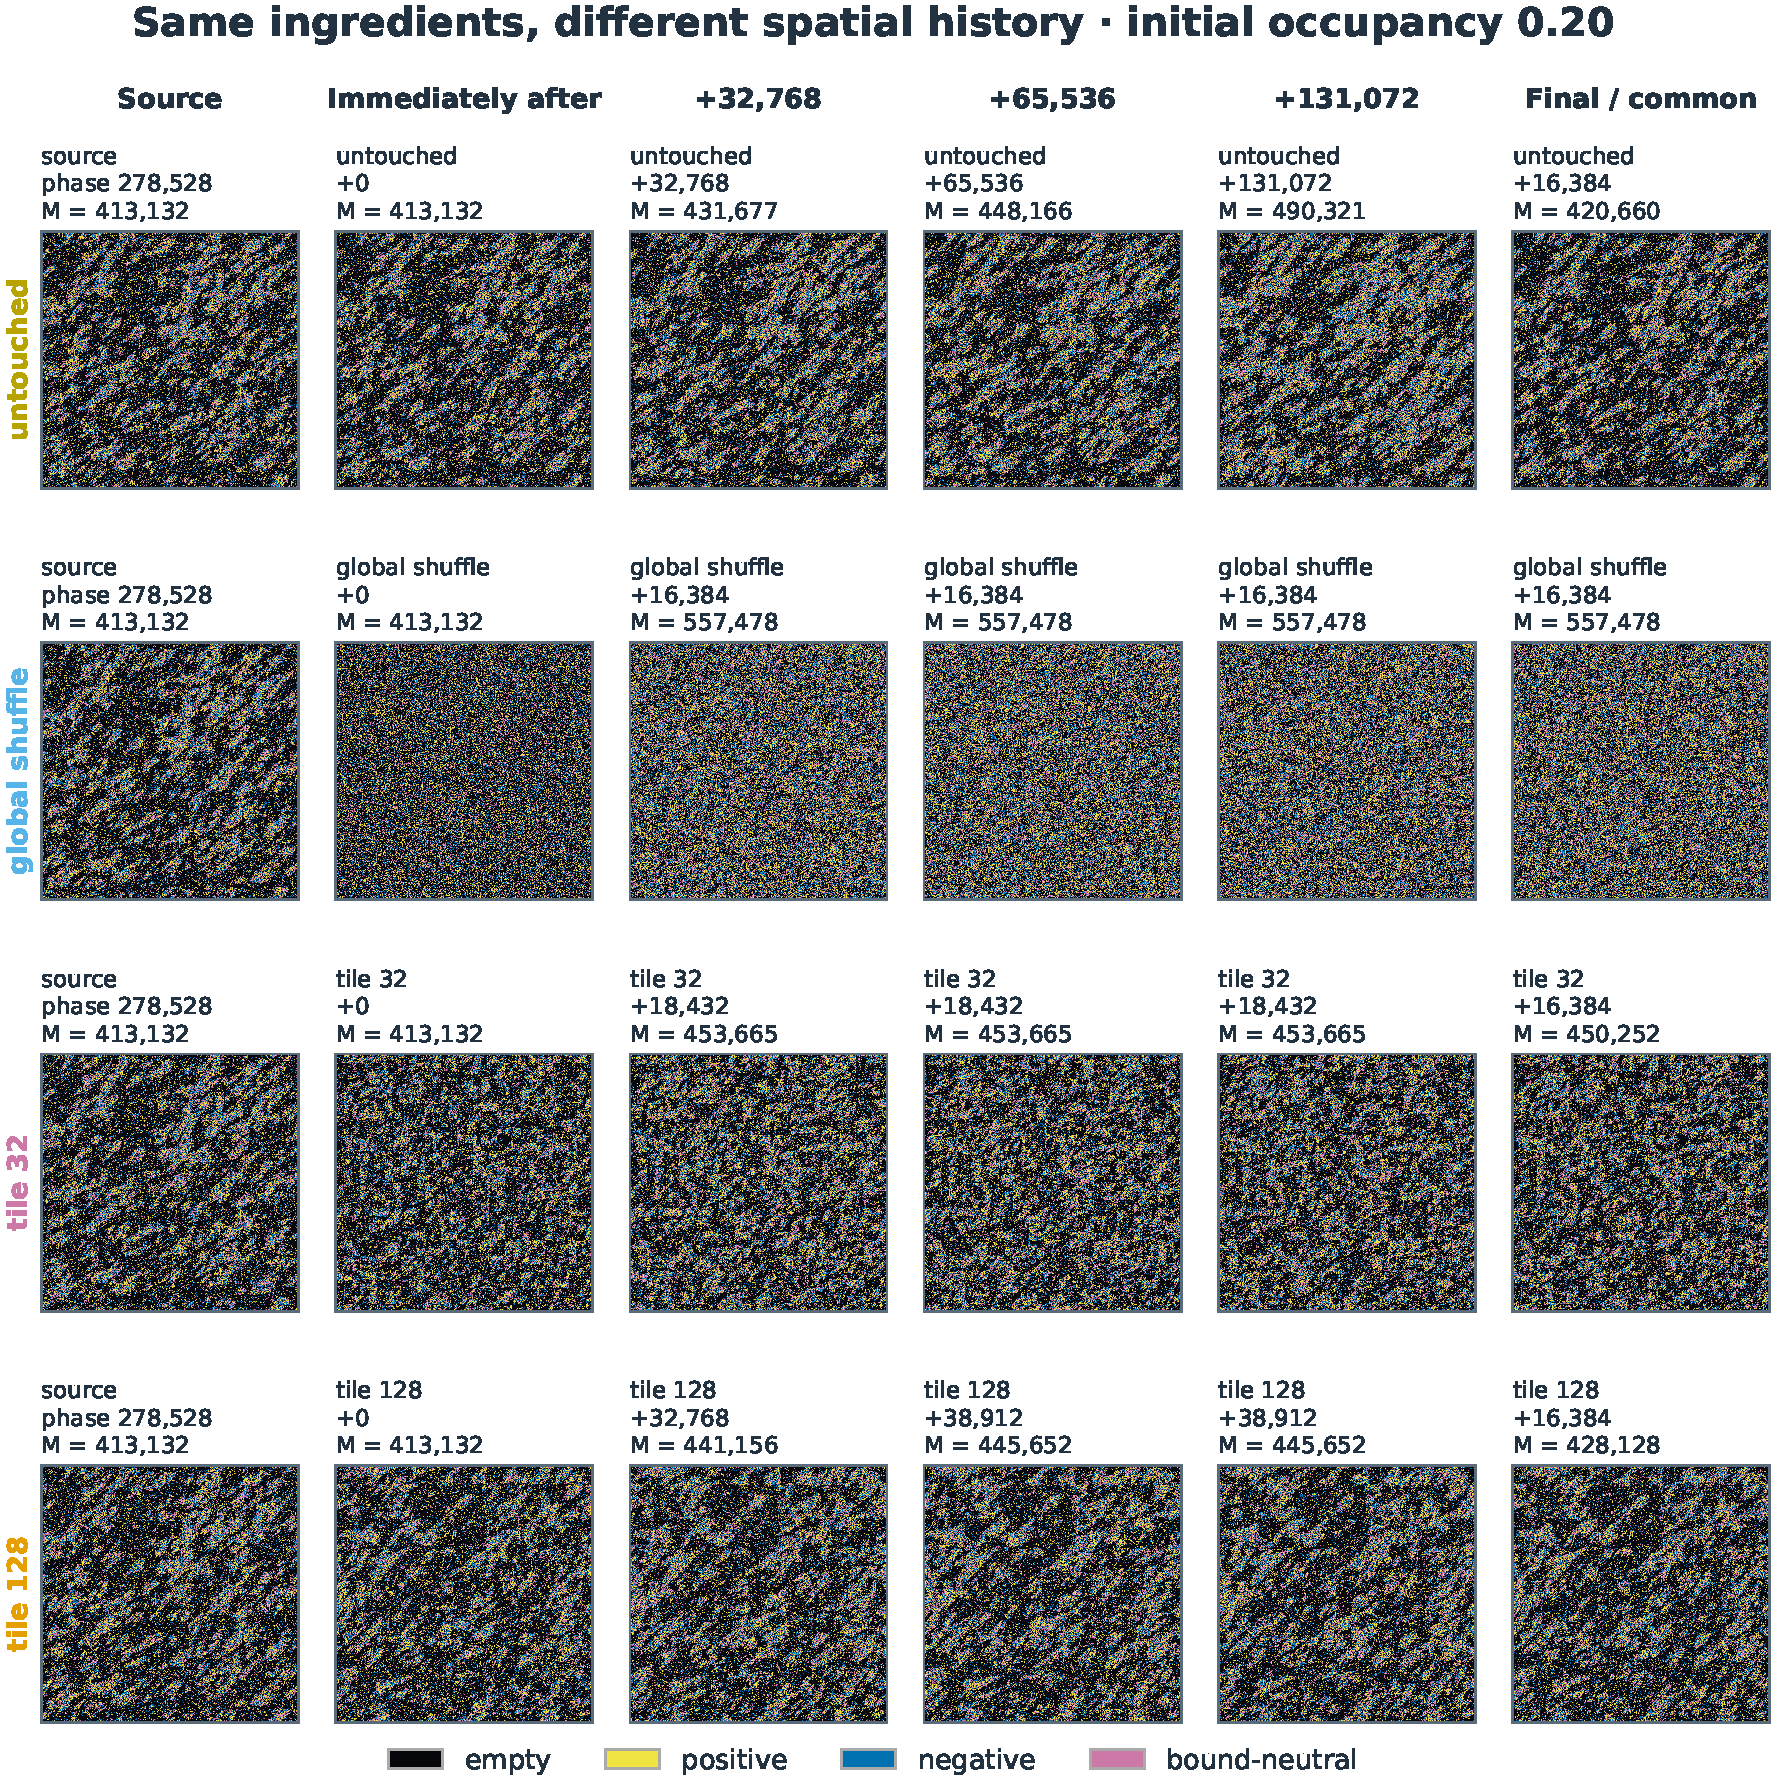
\includegraphics[scale=0.5]{FIGURE_02A_HISTORY_ERASURE_BRANCHES_V135.pdf}
\caption{\textbf{The same ingredients, rearranged.} Rows: untouched, global shuffle, and $32\times32$ and $128\times128$ tile permutations, at initial occupancy 0.20. Columns: the source, immediately after the intervention, then stored states. Headings give requested offsets; panel labels give actual offsets. Terminal states repeat when a branch ends before a requested offset, and the last column compares all branches at their largest common offset. Below, $32\times32$-cell details of the source and the shuffled state show the four cell states. The 0.24 source follows.}
\end{figure}

\begin{figure}[p]
\ContinuedFloat
\centering
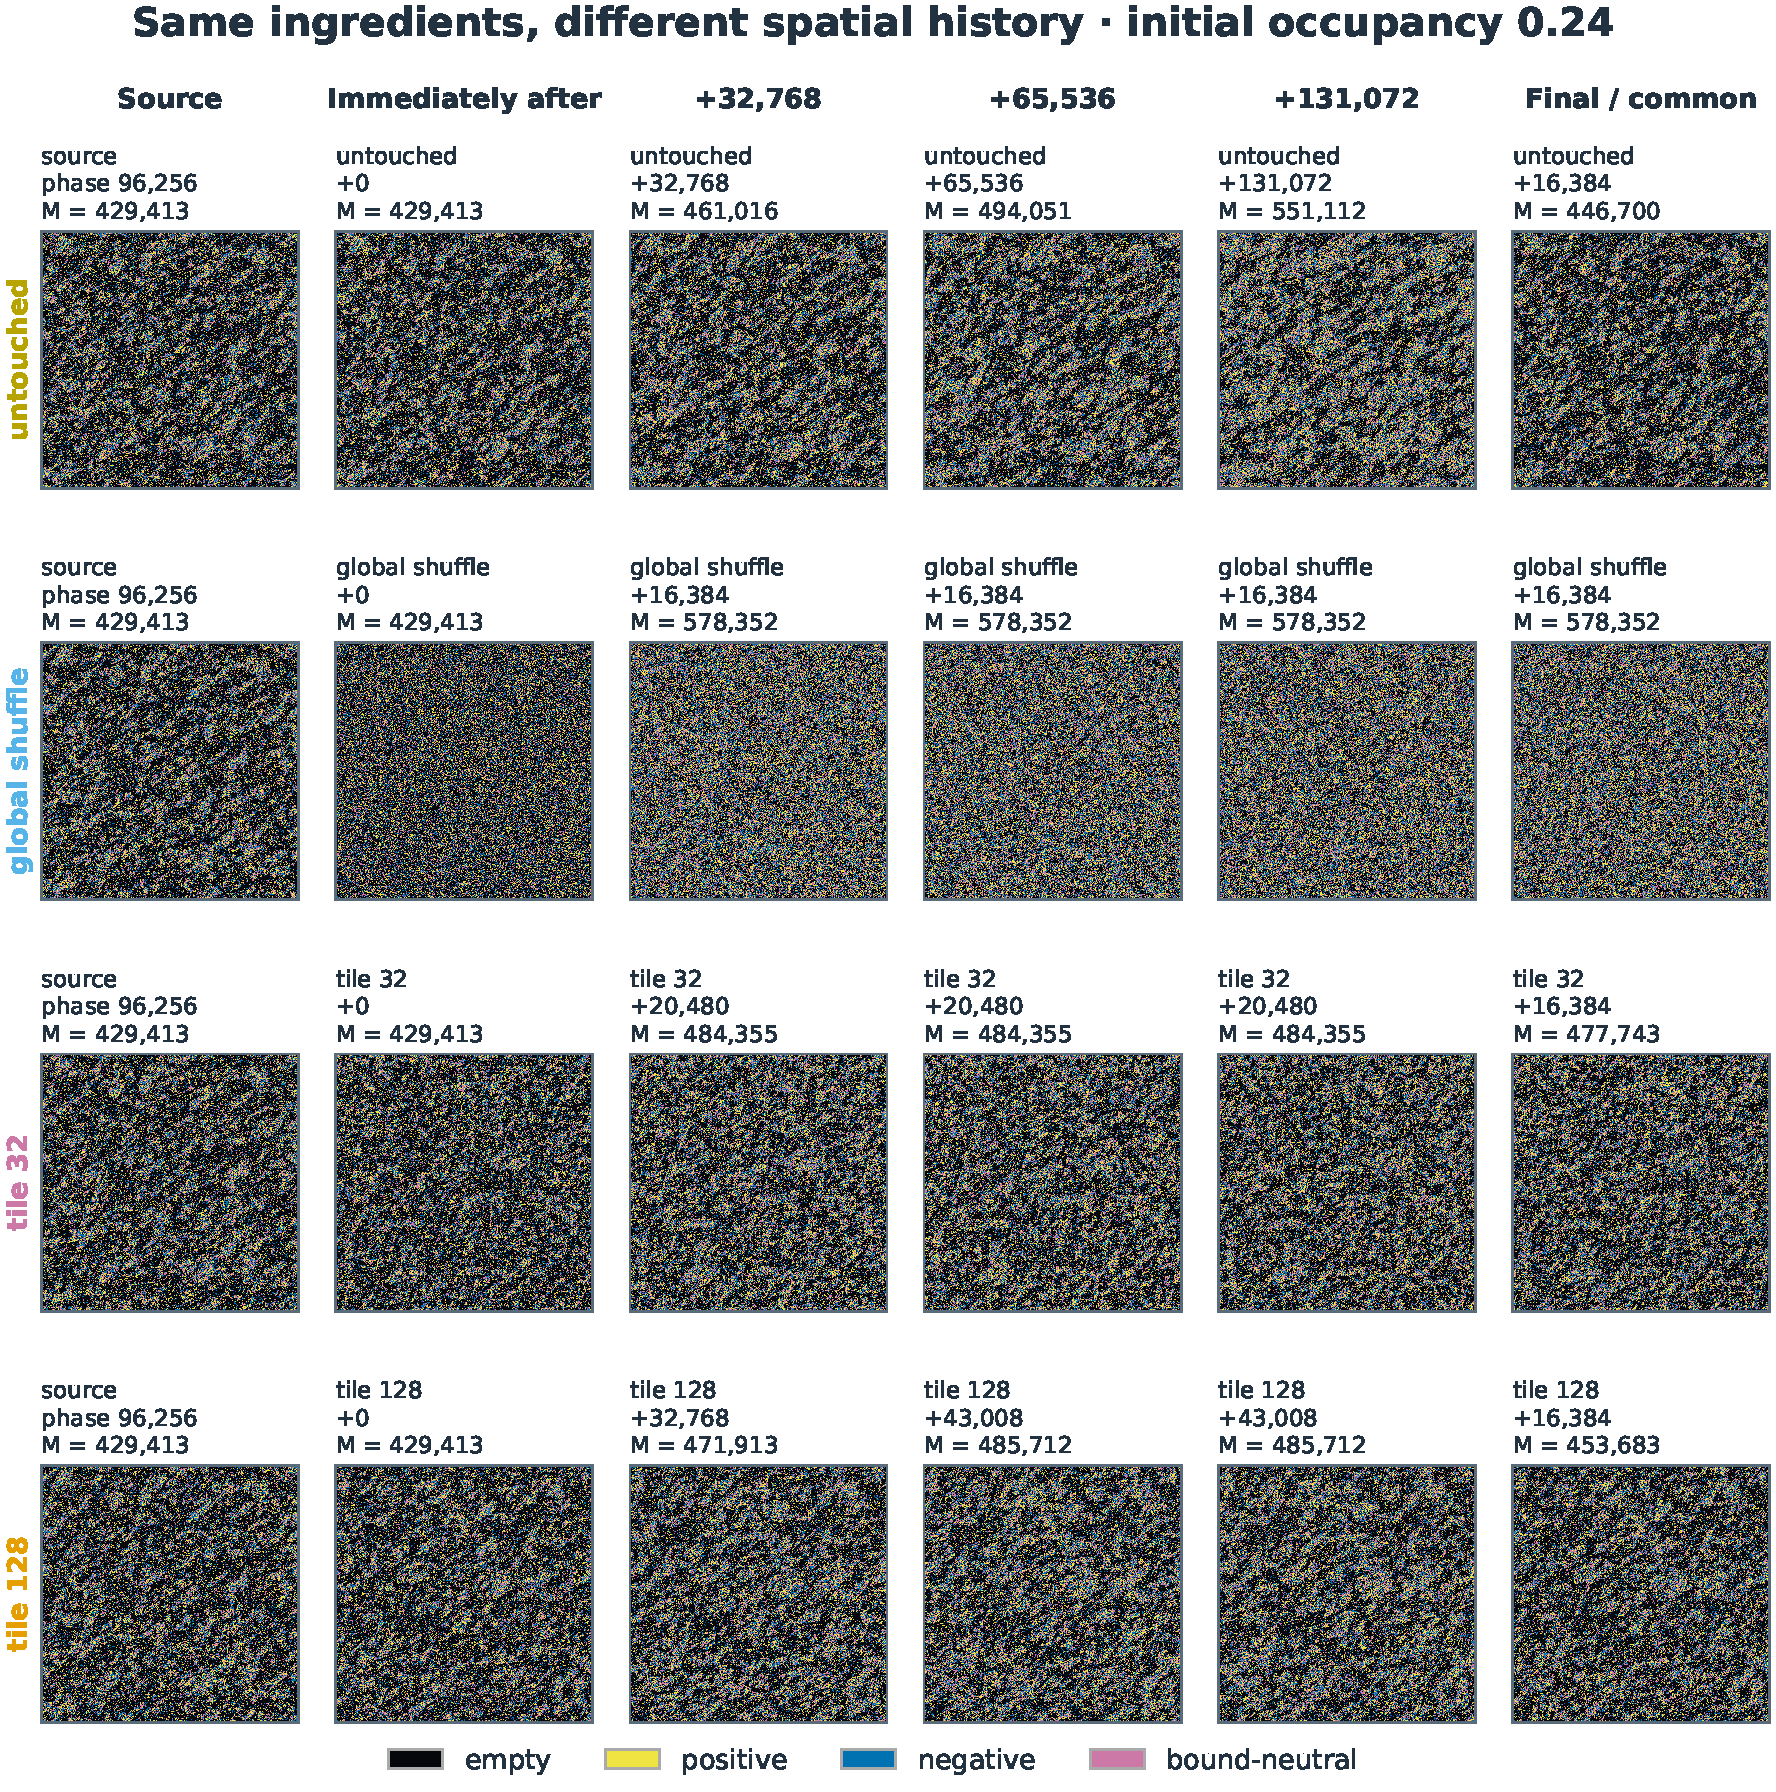
\includegraphics[scale=0.5]{FIGURE_02B_HISTORY_ERASURE_BRANCHES_V135.pdf}
\caption{\textbf{Continued: the source at initial occupancy 0.24.} Rows, columns and labels as on the previous page. Where a branch's stored states end before a requested offset, its panels give the offset actually reached, and the last column again shows every branch at the largest offset all four reached.}
\end{figure}

\begin{figure}[p]
\centering
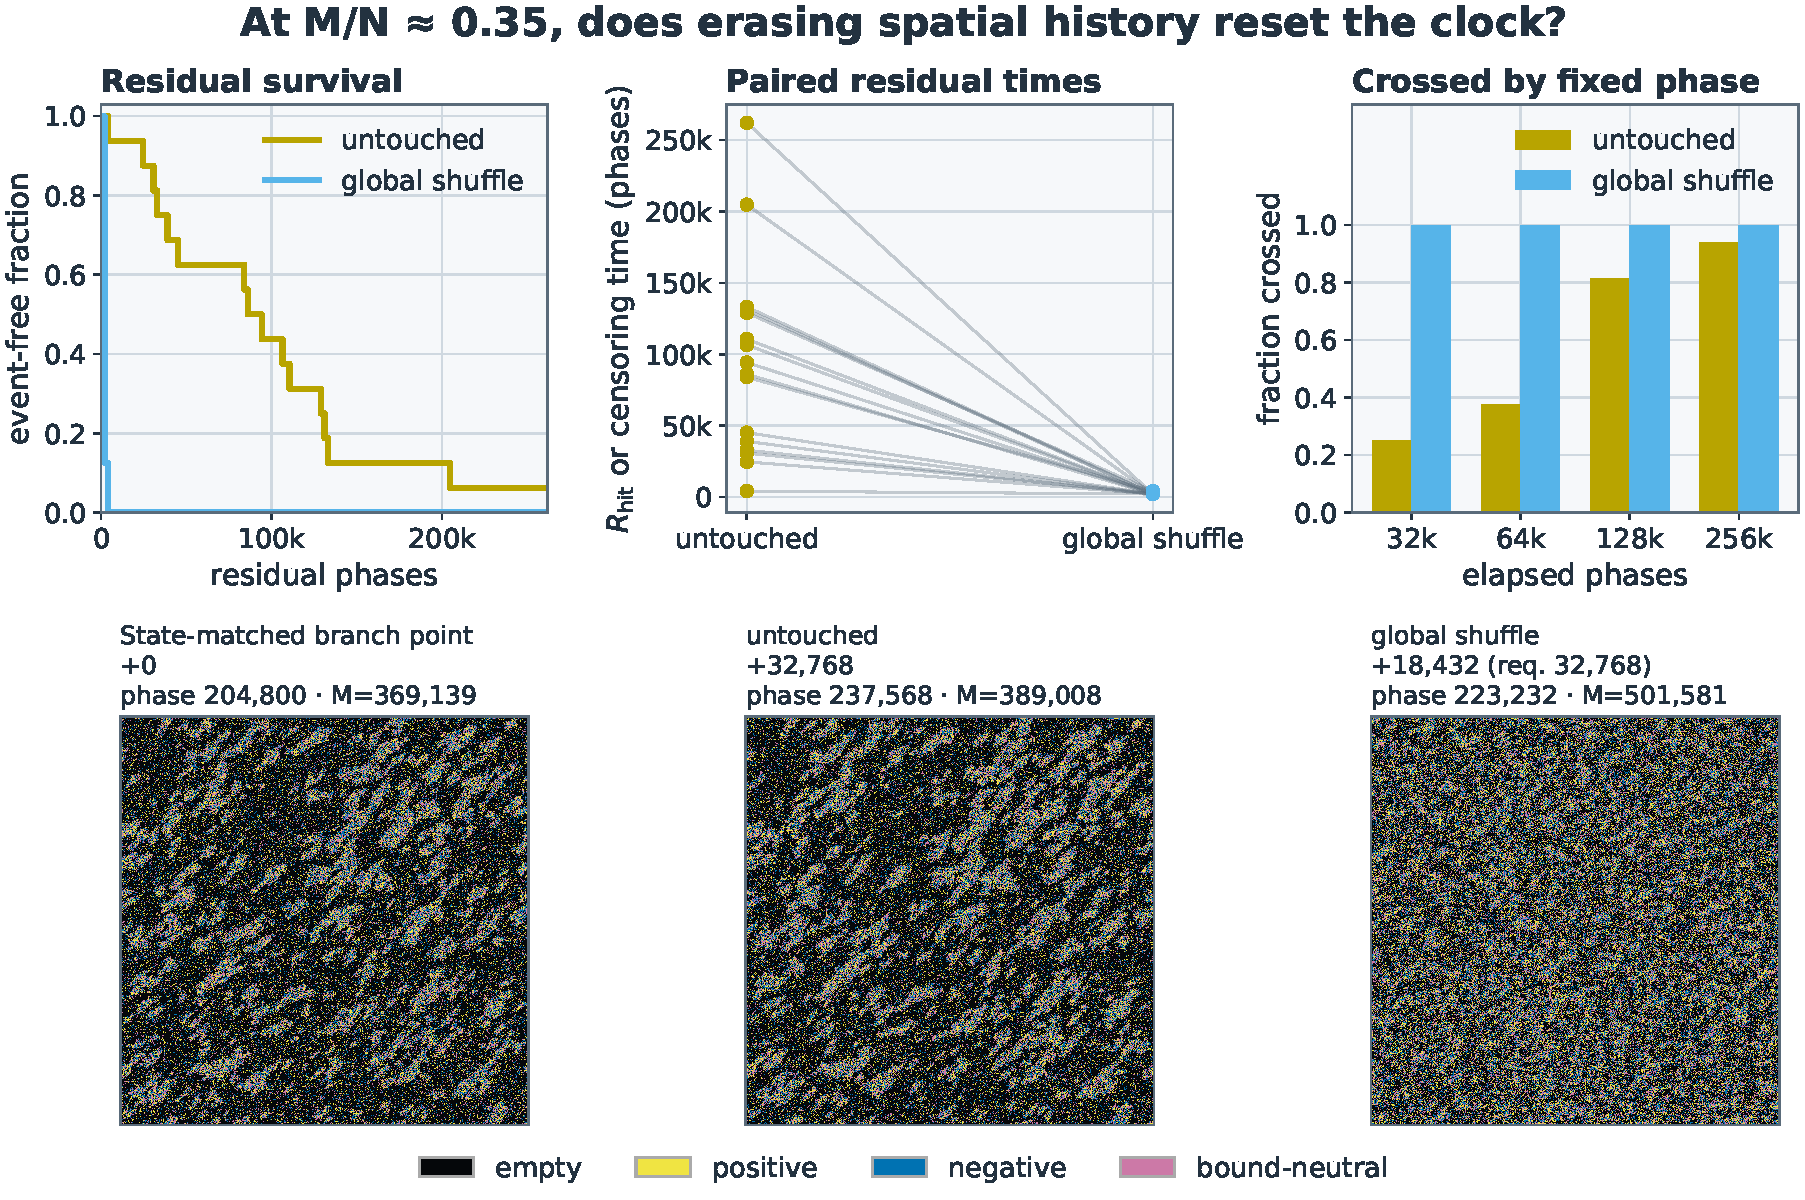
\includegraphics[scale=0.5]{FIGURE_03_FIXED_OCCUPANCY_HISTORY_ERASURE_V135.pdf}
\caption{\textbf{Fixed-occupancy branching.} Branch A at $M/N\geq0.35$. Upper plots: residual first-passage survival, paired residual times, and the fraction crossed by elapsed phase. Lower row: the branch-point state, the untouched continuation and the global shuffle. The shuffle panel is a terminal stored state; its actual offset differs from the requested one.}
\end{figure}

\begin{figure}[p]
\centering
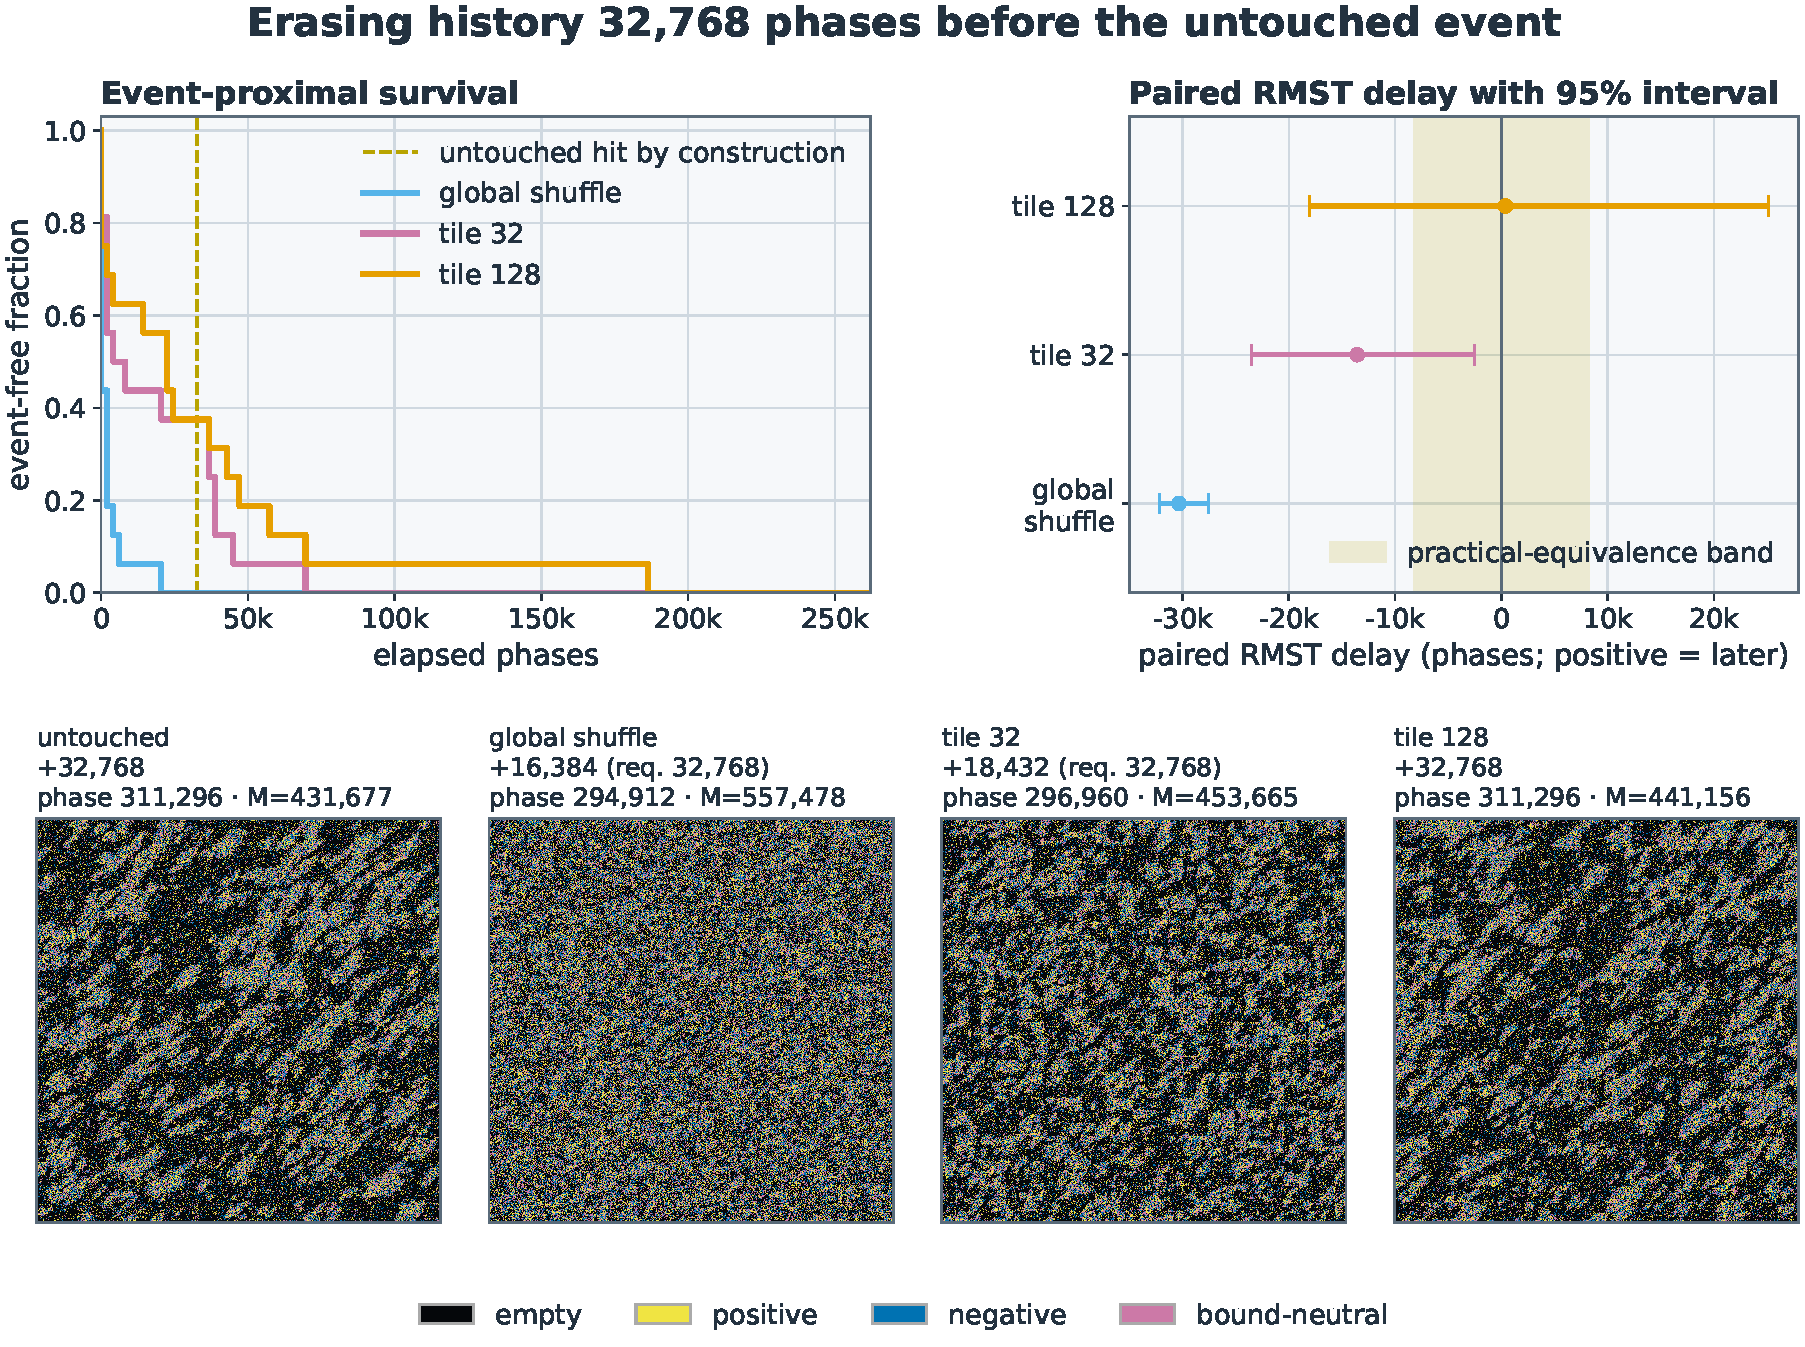
\includegraphics[scale=0.5]{FIGURE_04_EVENT_PROXIMAL_HISTORY_ERASURE_V135.pdf}
\caption{\textbf{Event-proximal branching.} Branch B starts 32,768 phases before the untouched first hit, marked by the dashed line. Upper right: paired differences in restricted mean survival time (RMST) against the untouched arm, with 95\% intervals and a practical-equivalence band; positive means later. Lower panels show different elapsed times; the global-shuffle and tile-32 panels are terminal stored states.}
\end{figure}

\begin{figure}[p]
\centering
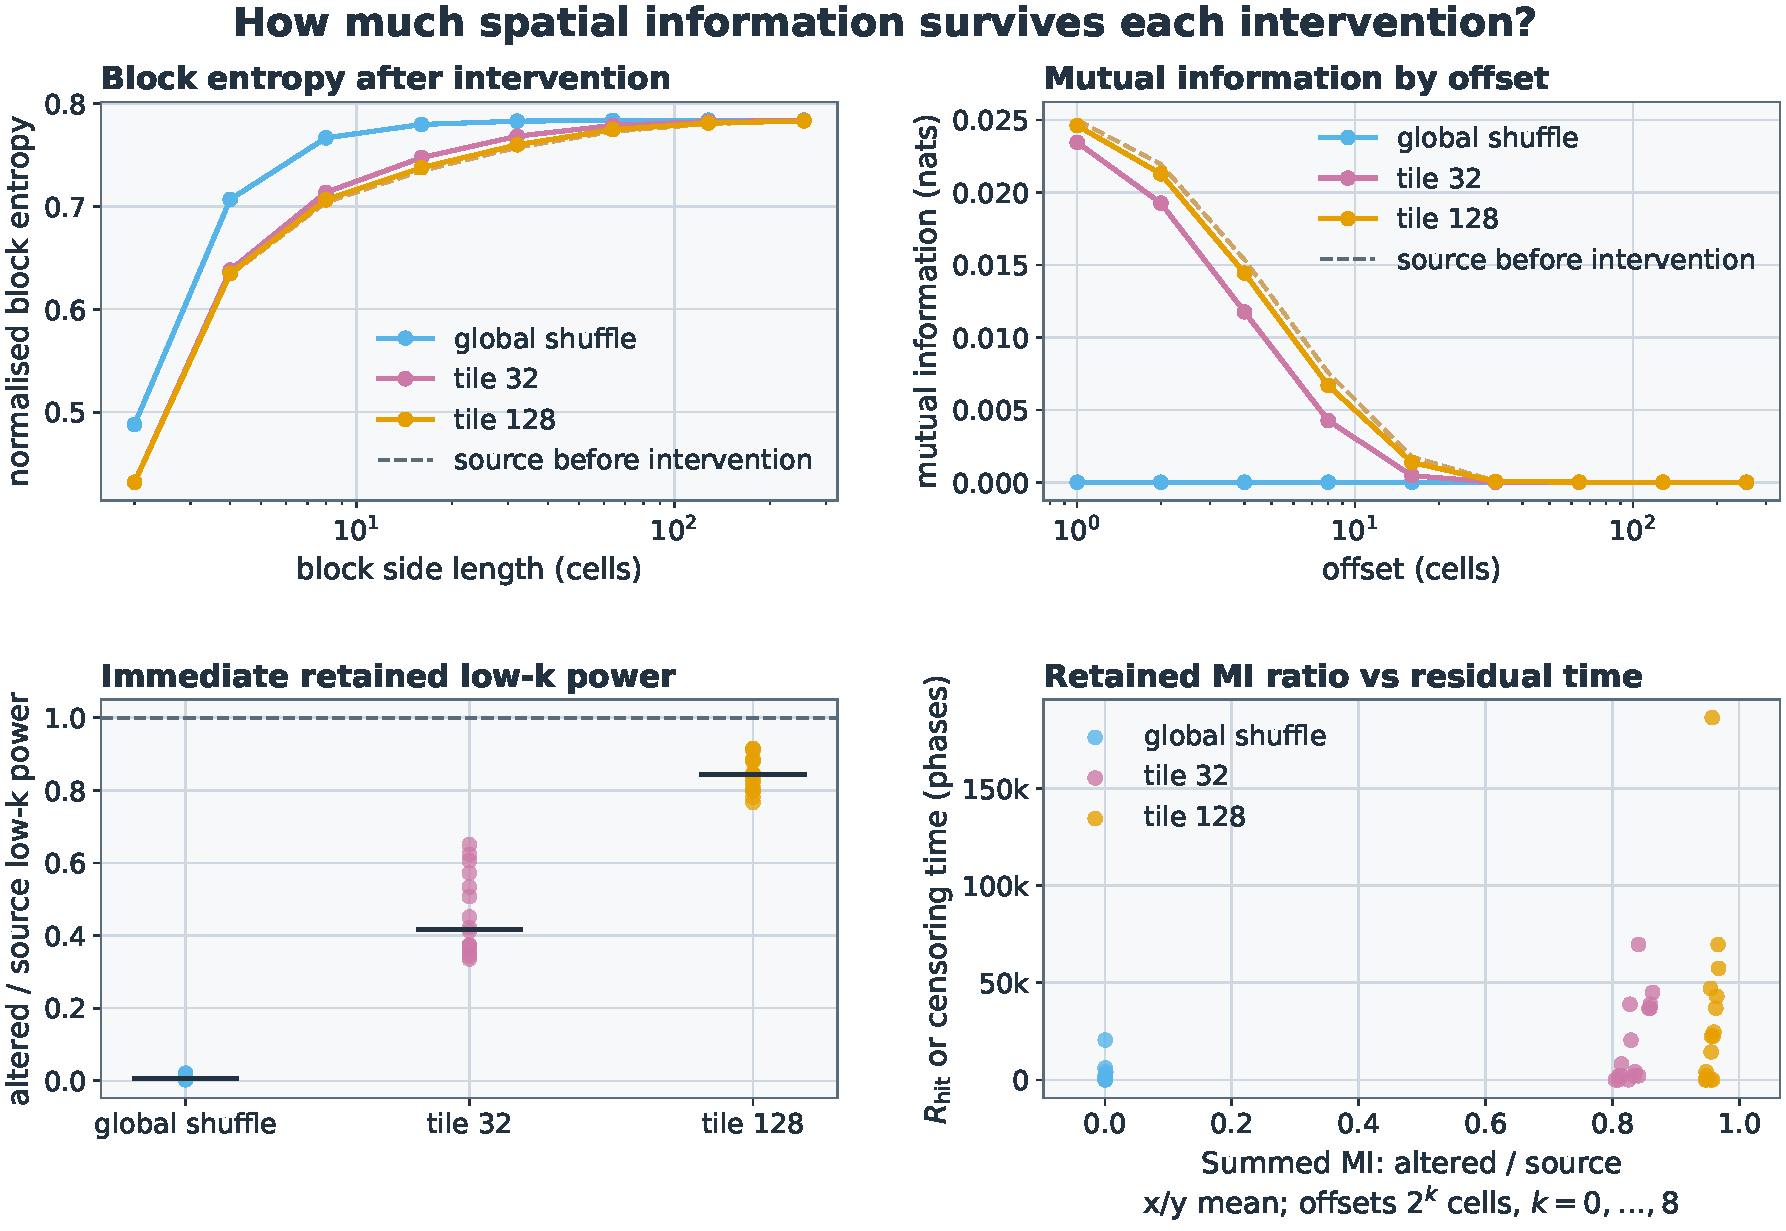
\includegraphics[scale=0.5]{FIGURE_05_MULTISCALE_MEMORY_V135.pdf}
\caption{\textbf{Spatial information after intervention.} Upper left: mean normalised Shannon entropy of the four-state fractions within non-overlapping blocks. Upper right: mutual information between cell states by distance. Solid curves show altered states and dashed curves their sources; lines join measurements. Lower left: retained over source long-wave power, one point per replicate, bars at medians. Lower right: residual time against the share of the source's mutual information kept, summed over the nine distances before dividing.}
\end{figure}

\begin{figure}[p]
\centering
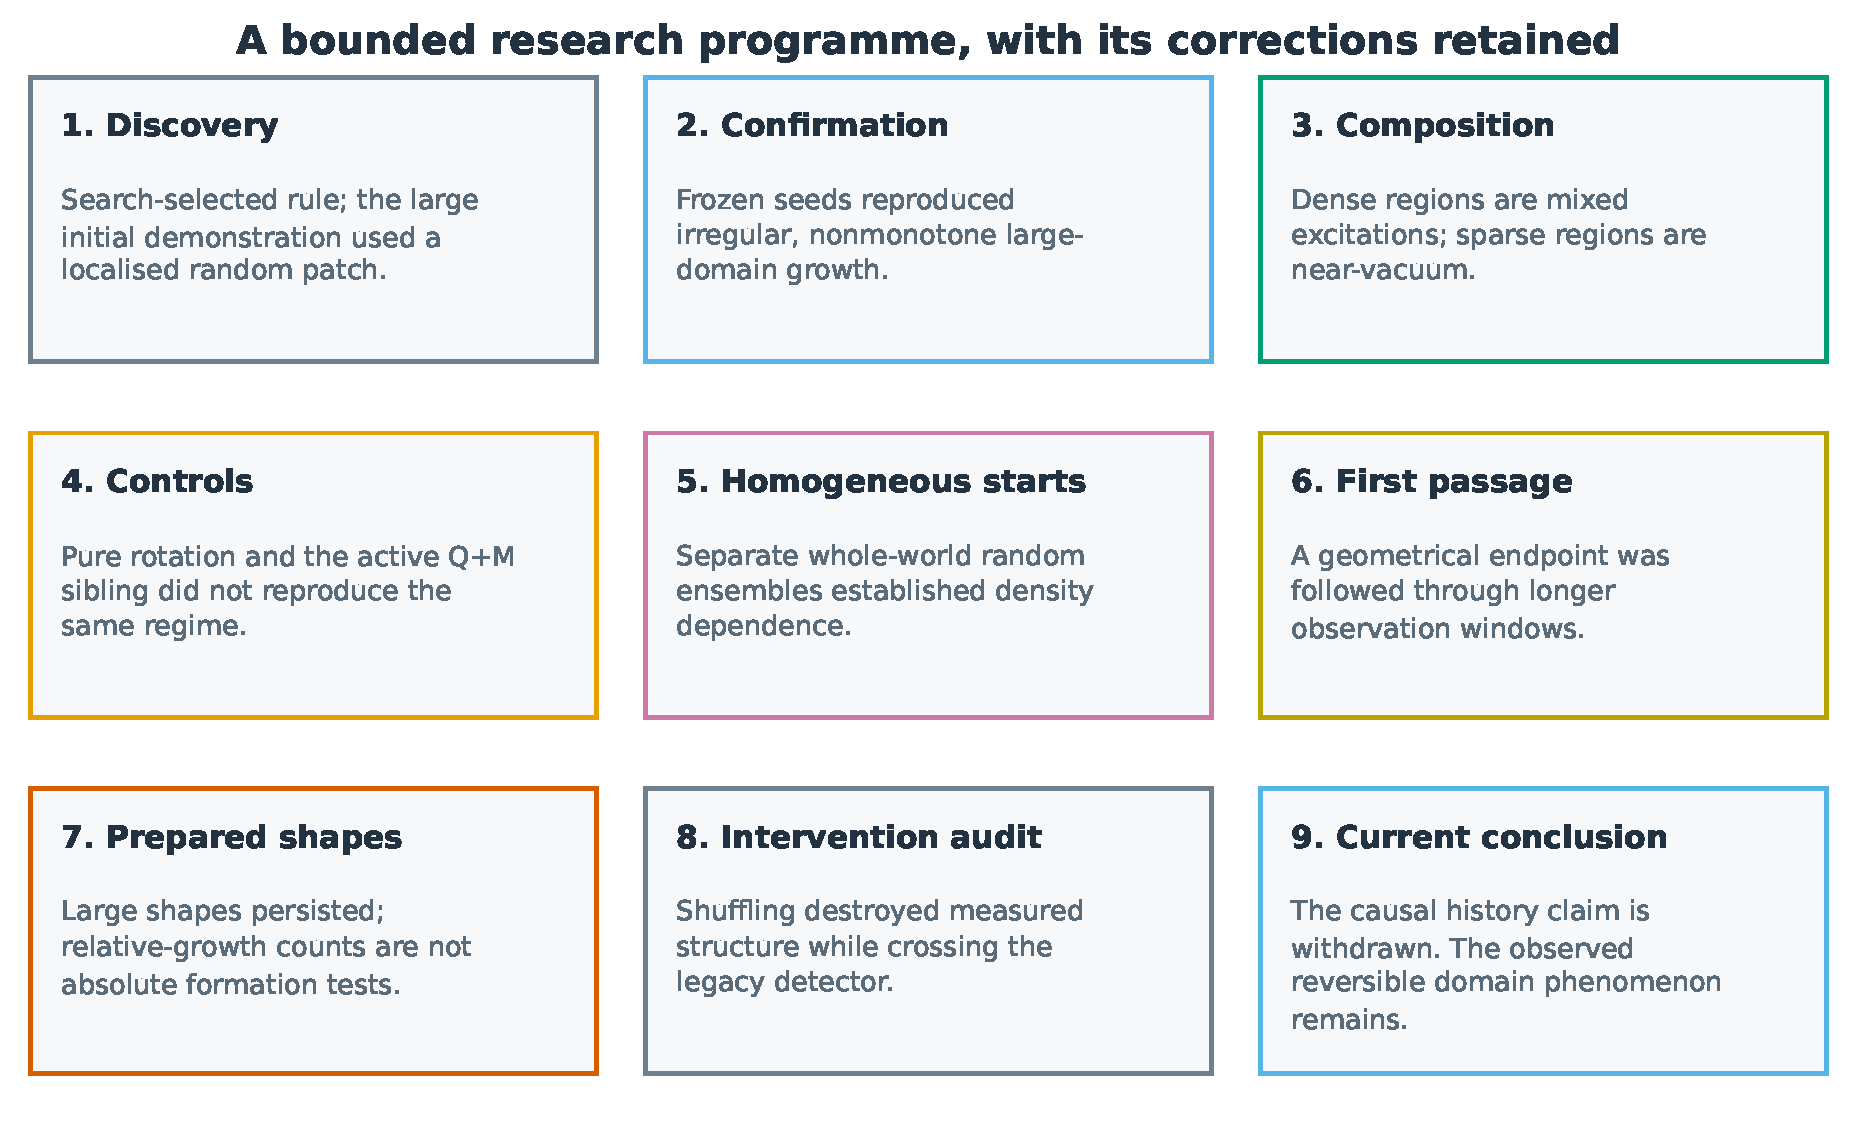
\includegraphics[scale=0.5]{COMPANION_V135_FIGURE_08_CORRECTED_RESEARCH_STORY.pdf}
\caption{\textbf{The evidence, from selection to the shuffling test.} The nine boxes run from the selective search to the shuffling test: the selective discovery search, the frozen-rule confirmations and the composition result, then the controls, the homogeneous-start ensembles, first passage and the prepared-shape comparison, and last the intervention audit and what survives it. The final box states the current position: the shuffling test cannot support a causal history claim, while the directly measured reversible domain formation remains. This is an explanatory summary of studies reported elsewhere in this Supplement, not an additional measurement.}
\end{figure}

\section{Prior-art positioning}
Reversible block automata and conservative logic are foundational precedents \citep{FredkinToffoli1982,Margolus1984,ToffoliMargolus1987}. Lattice gases provide exact local collision and transport frameworks \citep{HPP1973,FrischHasslacherPomeau1986,RothmanZaleski1994,BoonEtAl1996}, and reversible lattice-gas work directly addresses macroscopic irreversibility under microscopically reversible dynamics \citep{Broadwell2001}. Q2R models provide reversible conservative statistical dynamics \citep{Takesue1987,UrbinaRica2016,Urbina2020}; reversible aggregation provides an especially close visual and mechanistic neighbour \citep{DSouzaMargolus1999}. Reversible number-conserving automata and partitioned constructions further narrow the architectural context \citep{BoccaraFuks2002,MoritaImai2001}. Two-species reversible automata with vacancies, reactions and multiple local charges are close modern neighbours \citep{MedenjakPopkovProsen2019,KlobasProsen2022}; reactive lattice-gas waves and Turing patterns provide a non-reversible pattern-forming comparison \citep{KapralLawniczakMasiar1991}. The prior-art review and comparison matrix are in \code{paper/prior\_art}.

The residual contribution is the combination, not any isolated ingredient: an exact four-state signed invariant with variable occupancy; delayed distributed coarsening-like organisation; exact large-lattice reversal; density and waiting-time characterisation; and a hierarchy of geometry, double-conservation, and reaction controls. The review does not claim exhaustive priority.

\section{Reproducibility, hashes, and archive policy}
The public release contains compact result tables, reports, the figures used by the paper, rule files and provenance records; its \code{MANIFEST.csv} gives the size and SHA-256 digest of every included file. Large raw trajectories, checkpoints and full-resolution state arrays are retained by the author and are named by hash in the campaign records.

\textbf{Independent parity oracle.} The frozen rule and the Margolus update were re-implemented in Eshkol~\citep{Tsotchke2026Eshkol} (version 1.3.4-evolve), a Scheme-based language compiled to native code via LLVM. The Python package generates a self-contained Eshkol program that re-runs the exhaustive 256-entry audit (output range, one-to-one outputs, exact local charge) and replays a $16\times16$ exact-inventory torus (initial occupancy 0.28, seed 303) for 256 phases (one partition phase per step); the Python simulator's expected final lattice is stored beside the source and every cell is compared. The recorded run reports \code{AUDIT\_OK}, zero mismatched cells, and exact agreement in $Q=0$ and $M=97$. The generated program, the expected lattice and the recorded result ship in the release under \path{extensions/reversible_null_phase/eshkol/}.

\begingroup\sloppy The release includes the raw intervention results and the classifier diagnostics.\par\endgroup

The archived release is deposited at Zenodo, DOI \href{https://doi.org/10.5281/zenodo.22270456}{\mbox{10.5281/zenodo.22270456}}.

\footnotesize
\bibliographystyle{unsrtnat}
\bibliography{references}
\end{document}
